% !TEX root = Theo_III.tex
\chapter{Magnetostatik}


In den vorigen Kapiteln haben wir uns mit der Elektrostatik beschäftigt und gesehen, wie Ladungen dem Coulombgesetz gehorchen und ein elektrisches Feld hervorrufen, das die Grundgleichungen $\rot \vec {E}=0$ und $\divg \vec {D}=0$ erfüllt.

In der Magnetostatik betrachten wir jetzt stationäre (also nicht zeitabhängige) Ströme und die Kraftwirkung, die sie hervorrufen. Es wird ein Magnetfeld und die Stromdichte eingeführt, was schließlich auf eine integrale und differentielle Formulierung der Grundgesetze der Magnetostatik führt.

Es gibt Ähnlichkeiten zwischen der Elektro- und Magnetostatik, wie zum Beispiel das Abstandsverhalten und die Symmetrie einiger Formeln, aber auch wesentliche Unterschiede, unter Anderem in den Kraftrichtungen und Potentialen.

\section{Strom, Stromdichte und Kontinuitätsgleichung}

Der elektrische Strom $I$ ist als zeitliche Änderung der Ladung definiert,
\begin{equation*}
	I=\frac{\diff q}{\diff t}.
\end{equation*}
Die Einheit ist der Ampère. Aus der Ladungserhaltung folgt, dass der Strom konstant entlang eines Drahts ist.

Außerdem wird die Stromdichte als Strom pro Querschnittsfläche $A$
\begin{equation*}
	\vec {j}=\frac{\text{Strom}}{\text{Fläche}}=\frac{I}{A}\frac{\diff \vec {\vec {r}}}{\diff s}\:\xrightarrow{\Delta  f\diff s=\diff ^{3}r}\: \vec {j}\diffa[3]{\vec{r}}=I\diff \vec {r}
\end{equation*}
definiert. Dabei ist $\diff\vec r$ als Leiterelement und $I\diff\vec r$ als gerichtetes Stromelement zu verstehen. Es gilt also
\begin{equation*}
	I=\int_A \vec j \cdot \diff \vec A,
\end{equation*}
bzw. für eine gleichmäßig auf $A$ verteilte Stromdichte
\begin{equation*}
	I=\vec j\cdot \vec A.
\end{equation*}

Die Stromdichte lässt sich auch ausdrücken durch das Produkt aus Ladungsdichte und Geschwindigkeit,
\begin{equation*}
	\vec {j}=\rho \vec {v},
\end{equation*}
was eine mikroskopische Definition analog zu der der Ladungsdichte erlaubt\footnote{Zur Erinnerung: $\rho =\sum _{i}q_{i}\delta \left(\vec {r}-\vec {r}_{i}\right)$.}:
\begin{equation*}
	\vec {j}=\sum _{i}q_{i}\vec {v}_{i}\delta \left(\vec {r}-\vec {r}_{i}\right)
\end{equation*}
Die Stromdichte zeigt damit in dieselbe Richtung wie der Geschwindigkeitsvektor einer positiven Ladung.

Zur Herleitung der Kontinuitätsgleichung betrachten wir die zeitliche Änderung der Ladung in einem Volumen $V$:
\begin{equation*}
	\frac{\diff Q}{\diff t}=\frac{\diff }{\diff t}\int _{V}\diff^{3}\vec {r}\rho \left(\vec {r},t\right)=\int _{V}\diffa[3]{\vec{r}}\frac{\partial }{\partial t}\rho \left(\vec {r},t\right)
\end{equation*}
Wegen der Ladungserhaltung entspricht dies gerade dem Fluss der Stromdichte aus der Volumenoberfläche $\partial V$ heraus:
\begin{equation*}
	\int _{V}\diffa[3]{\vec{r}}\frac{\partial }{\partial t}\rho \left(\vec {r},t\right)=-\int _{\partial V}\vec {j}\cdot \diff \vec {f}=-\int _{V}\diffa[3]{\vec{r}}\divg \vec {j},
\end{equation*}
woraus sich die Kontinuitätsgleichung ergibt:
\begin{equation*}
	\frac{\partial }{\partial t}\rho +\divg \vec {j}=0
\end{equation*}
In der Magnetostatik ist $\partial _{t}\rho =0$ und damit
\begin{equation*}
	\divg \vec {j}=0.
\end{equation*}
\section{Leiter und Magnetfeld}

Auf Erde kommen im Wesentlichen zwei natürliche bekannte Magnetfelder vor: dasjenige der Erde und das Magnetfeld von speziellen Mineralen, wie zum Beispiel Magnetit. Hans Christian \O{}rsted entdeckte im 19. Jahrhundert, dass auch stromdurchflossene Leiter ein Magnetfeld erzeugen und André-Marie Ampère entdeckte fast zeitgleich, dass ein Magnetfeld eine Kraftwirkung auf Leiter hervorruft.

Auf ein stromdurchflossenes Volumenelement $\diff V=\diff^3 \vec r$ in einem Magnetfeld $\vec B$ wirkt nach dem folgenden Gesetz eine Kraft\footnote{vergleichlich mit $\vec {F}=q\vec {E}$, also Produkt aus Quelle und Feld in der Elektrostatik. }:
\begin{equation*}
	\diff \vec {F}=(\vec j\times\vec B)\diff V
\end{equation*}
Die Gesamtkraft auf einen ausgedehnten Leiter $V$ ergibt sich durch Integration:
\begin{equation*}
	\vec {F}=\int _{V}\vec {j}\times \vec {B}\diff V
\end{equation*}
Im Spezialfall für einen dünnen Leiter $C$ und ein Leiterelement $\diff\vec r$ ($\diff V = \diff A\diff\vec r$) gilt
\begin{align}
	\label{eq:def_magn_flussdichte}
	\diff \vec F & =I\diff\vec r\times\vec B                                                                                               \\
	\vec {F}     & =\int _{V}\vec {j}\times \vec {B}\diff A \diff\vec r = \int_{A}j\diff A \cdot \int_C \diff\vec r\times \vec B \nonumber \\& = I\int_C \diff\vec r\times \vec B .\nonumber
\end{align}

\begin{figure}[htb]
	\centering
	\tfigMagnetfeldBeiLeiter
	\caption{Stromelement $I\diff\vec r$ und Magnetfeld $\vec B$ eines Leiterelements $\diff \vec r$. }
	\label{fig:magnetic_field_conductor_diff_view}
\end{figure}
Wir untersuchen zunächst die magnetische Flussdichte einiger speziellen geometrischen Anordnungen. Es gilt für ein Leiterelement $\diff \vec {r}'$ (dargestellt in \Abbref{fig:magnetic_field_conductor_diff_view}):
\begin{equation*}
	\diff \vec {B}=\frac{\mu _{0}}{4\pi }I\diff \vec {r}'\times \frac{\vec {r}-\vec {r}'}{\left| \vec {r}-\vec {r}'\right| ^{3}}
\end{equation*}
Dieser Zusammenhang ist als Biot-Savartsches Gesetz für Leiter bekannt und ergibt sich aus den Betrachtungen $\left| \diff \vec {B}\right| \propto I\left| \diff \vec {r}'\right| , \left| \vec {r}-\vec {r}'\right| ^{-2}$ und $\diff \vec {B}\perp \diff \vec {r}',\vec {r}-\vec {r}'$. Hier wird außerdem die magnetische Feldkonstante $\mu _{0}\approx 4\pi \cdot 10^{-7}\,\si{\newton\per\square\ampere}$ eingeführt\footnote{Über die Kraft zwischen zwei stromdurchflossene parallele Leiter wurde früher die Einheit Ampère definiert und dabei festgelegt, dass $\frac{\mu _{0}}{4\pi }=\SI{1e-7}{\newton\per\square\ampere}$, aber die magnetische Feldkonstante wurde 2019 umdefiniert auf Basis der Elementarladung und Sekunde, wobei aber die Abweichung extrem gering ist. Damit ist die magnetische Feldkonstante eine experimentell zu ermittelnde Größe geworden. }. Die Flussdichte ist zwar proportional zu $r^{-2}$ wie beim elektrischen Feld einer Punktladung, aber im Gegensatz können isolierte Stromelemente $I\diff \vec {r}$ nicht existieren.

Für das Feld eines unendlich langen, geraden Leiters gilt
\begin{equation}
	\label{eq:biot_savart}
	B\left(\rho \right)=\frac{\mu _{0}}{4\pi }I\rho \int _{-\infty }^{\infty }\frac{\diff z}{\left(\rho ^{2}+z^{2}\right)^{\frac{3}{2}}}=\frac{\mu _{0}}{2\pi }\frac{I}{\rho },
\end{equation}


\begin{figure}[htb]
	\centering
	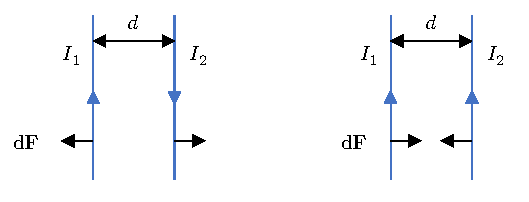
\includegraphics{force_parallel_conductors.pdf}
	\caption{Die Kraft auf parallele, stromdurchflossene Leiter ist anziehend, wenn der Stromfluss in verschiedene Richtungen geht und abstoßend, wenn der Strom in beiden Leiter in der gleichen Richtung fließt. }
	\label{fig:force_parallel_conductors}
\end{figure}

Diese Gleichung beschreibt das historische Biot-Savartsche Gesetz.

Verwendet man Gleichungen \eqref{eq:def_magn_flussdichte} und \eqref{eq:biot_savart}, so erhält man die Kraft zwischen zwei parallelen Leitern mit Abstand $d$ (siehe \Abbref{fig:force_parallel_conductors})
\begin{equation*}
	\frac{\diff\vec F}{\diff z} = \frac{\mu_0}{2\pi} \frac{I_1I_2}d,
\end{equation*}
die orthogonal zum Leiter ist.

Bis zum 20.5.2019 war der Ampère definiert als der Strom, der durch zwei parallele Leiter der Länge $\SI{1}{\m}$ mit $\SI{1}{\m}$ Abstand in gleicher Richtung fließt und eine Anziehungskraft von $\SI{1e-7}{\newton}$ bewirkt.

Heute gilt
\begin{equation*}
	\SI{1}{\ampere}\equiv \frac{\SI{1}{\coulomb}}{\SI{1}{\s}}.
\end{equation*}
Zwischen beliebigen Leiterschleifen $C_{1},C_{2}$ wirkt eine Kraft von
\begin{equation*}
	\vec {F}_{21}=-\vec {F}_{12}=-\frac{\mu _{0}}{4\pi }I_{1}I_{2}\oint _{C_{1}}\oint _{C_{2}}\frac{\vec {r}_{1}-\vec {r}_{2}}{\left| \vec {r}_{1}-\vec {r}_{2}\right| ^{3}}\diff \vec {r}_{1}\cdot \diff \vec {r}_{2}.
\end{equation*}



\section{Grundgleichungen der Magnetostatik}

Um die Grundgleichungen der Magnetostatik herzuleiten, gehen wir zuerst von dem Stromelement $I\diff \vec {r}$ über in die Stromdichte $\vec {j}\left(\vec {r}\right)$ mit $I\diff \vec {r}=\vec {j}\left(\vec {r}\right)\diff^3 \vec {r}$.

Die Kraft auf ein Stromgebiet ist das Integral der Kraftdichte
\begin{equation*}
	\vec {F}=\int \vec f\left(\vec {r}\right)\diffa[3]{\vec{r}}=\int \vec {j}\left(\vec {r}\right)\times \vec {B}\left(\vec {r}\right)\diffa[3]{\vec{r}}.
\end{equation*}
Für eine Punktladung $q$, die sich mit Geschwindigkeit $\vec {v}$ bewegt ($\vec {j}=q\vec {v}\delta \left(\vec {r}-\vec {r}\left(t\right)\right)$) gilt speziell
\begin{equation*}
	\vec F\left(\vec {r}\right)=q\vec {v}\times \vec {B}\left(\vec {r},t\right)
\end{equation*}
bzw. allgemein mit einem zusätzlichen elektrischen Feld
\begin{equation*}
	\vec F\left(\vec {r}\right)=q\left(\vec {v}\times \vec {B}\left(\vec {r},t\right)+\vec {E}\left(\vec {r},t\right)\right).
\end{equation*}
Diese Gesamtkraft ist die sogenannte Lorentzkraft.

Integration des Biot-Savartschen Gesetzes für Leiter führt auf\footnote{vergleichlich mit $\vec {E}(\vec r)=\frac{1}{4\pi \varepsilon _{0}}\int \rho \left(\vec {r}\right)\frac{\vec {r}-\vec {r}'}{\left| \vec {r}-\vec {r}'\right| ^{3}}\diffa[3]{\vec{r}'}$.}
\begin{equation*}
	\vec {B}\left(\vec {r}\right)=\frac{\mu _{0}}{4\pi }\int \vec {j}\left(\vec {r'}\right)\times \frac{\vec {r}-\vec {r}'}{\left| \vec {r}-\vec {r}'\right| ^{3}}\diffa[3]{\vec{r}'}.
\end{equation*}
Wie für das elektrische Feld können wir ein Potential einführen \textendash{} allerdings ist $\vec {B}$ kein Potentialfeld und daher ist das magnetische Potential ein Vektorpotential:
\begin{equation*}
	\vec {B}\left(\vec {r}\right)=\nabla \times \vec {A}\left(\vec {r}\right), \quad\vec {A}\left(\vec {r}\right)=\frac{\mu _{0}}{4\pi }\int \frac{\vec {j}\left(\vec {r}'\right)}{\left| \vec {r}-\vec {r}'\right| }\diffa[3]{\vec{r}'}
\end{equation*}
Die Divergenz von $\vec {B}$ verschwindet, weil stets gilt, dass $\nabla\cdot(\nabla\times \vec A) = 0$.
\begin{formal}
	Das Magnetfeld hat keine Quellen, $\divg \vec {B}=0$.
\end{formal}
In der integralen Formulierung,
\begin{equation*}
	\int _{V}\divg \vec {B}\,\diffa[3]{\vec{r}}=\int _{\partial V}\vec {B}\cdot \diff \vec {f}=0,
\end{equation*}
bedeutet das, dass die magnetischen Feldlinien geschlossen sind. Es gibt folglich keine magnetischen Ladungen, wo die Feldlinien beginnen oder enden.

Für die Rotation der magnetischen Flussdichte gilt
\begin{align}
	\begin{split}
		\label{eq:durchflutungsgesetz_magnetostatik}
		\rot \vec {B}&=\nabla \times \left(\nabla \times \vec {A}\right)=\nabla \left(\nabla \cdot \vec {A}\right)-\nabla ^{2}\vec {A}\\
		&=\frac{\mu _{0}}{4\pi }\nabla \int \vec {j}\left(\vec {r}'\right)\cdot \nabla \frac{1}{\left| \vec {r}-\vec {r}'\right| }\diffa[3]{\vec{r}'}-\frac{\mu _{0}}{4\pi }\int \vec {j}\left(\vec {r}'\right)\nabla ^{2}\frac{1}{\left| \vec {r}-\vec {r}'\right| }\diffa[3]{\vec{r}'}\\
		&=0+\mu _{0}\int \vec {j}\left(\vec {r}'\right)\delta \left(\vec {r}-\vec {r}'\right)\diffa[3]{\vec{r}'}\\&=\mu _{0}\vec {j}\left(\vec {r}\right).
	\end{split}
\end{align}

\begin{formal}
	Elektrische Ströme rufen Wirbel in der magnetischen Flussdichte hervor, $\rot \vec {B}=\mu _{0}\vec {j}\left(\vec {r}\right)$.
\end{formal}
Alternativ kann man sagen, dass die Zirkulation entlang der Oberfläche eines Volumens einem Strom durch das Volumen entspricht,
\begin{equation*}
	\boxed{\int _{\partial F}\vec {B}\cdot \diff \vec {r}=\mu _{0}I.}
\end{equation*}
Diese Gleichung ist als Ampèresches Gesetz bekannt. Mit seiner Nutzung kann man leicht das Magnetfeld von einem homogen stromdurchflossenen, zylindrischen Draht mit Radius $R$ bestimmen, wie in Abbildung \Abbref{fig:cylinder_conductor_with_diagrams} gezeigt. Wähle dazu eine kreisförmige Kurve $C$ mit Radius $r$ um die $z$-Achse herum. Aufgrund der Zylindersymmetrie ist das Magnetfeld nur vom Abstand $r$ der $z$-Achse abhängig und es gilt mit dem Ampèreschen Gesetz
\begin{align*}
	B\left(r\right)\oint _{C}1\diff s & =2\pi rB\left(r\right)=\mu _{0}I\left(r\right) \\
	\equivalence B\left(r\right)      & =\frac{\mu _{0}I\left(r\right)}{2\pi r}.
\end{align*}


\begin{figure}[htb]
	\centering
	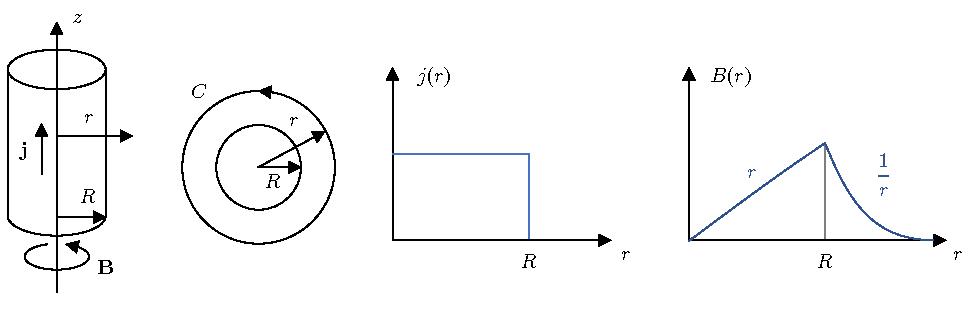
\includegraphics{cylinder_conductor_with_diagrams.pdf}
	\caption{Ein stromdurchflossener, zylindrischer Leiter mit Radius $R$ und Stromdichte $r$ erzeugt ein magnetisches Wirbelfeld. Links: schematische Darstellung, Mitte links: Querschnitt mit gedachter kreisförmiger Kurve $C$ mit Radius $r$ um den Leiter herum, Mitte rechts: Die Stromdichte ist konstant im Leiter und fällt außerhalb auf $0$ ab, rechts: im Leiter steigt der Betrag des Magnetfelds linear mit dem Abstand an und fällt außerhalb ab mit $r^{-1}$.  }
	\label{fig:cylinder_conductor_with_diagrams}
\end{figure}

Der Strom $I\left(r\right)$ enthält nur den Strom, der innerhalb der Kurve $C$ fließt. Innerhalb des zylindrischen Leiters ($r\leq R$) ist die eingeschlossene Fläche gerade $\pi r^{2}$ und damit
\begin{equation*}
	I\left(r\right)=j_{0}\pi r^{2}.
\end{equation*}


\begin{figure}[htb]
	\centering
	\tfigCoil
	\caption{Lange, stromdurchflossenen Spule. }
	\label{fig:long_coil_scheme}
\end{figure}

Außerhalb des Leiters ist $I$ konstant $j_{0}\pi R^{2}$, weil sich der Leiter und damit der Stromfluss nur bis $r=R$ erstreckt. Das Magnetfeld ist also
\begin{align*}
	B\left(r\right)=\frac{\mu _{0}}{2}j_{0}\begin{cases} r,               & r\leq R \\
              \frac{R^{2}}{r}, & r>R
	                                       \end{cases}
\end{align*}
und es ist kreisförmig um die $z$-Achse gerichtet, $\vec {B}\left(r,\varphi \right)=B\left(r\right)\vec {e}_{\varphi }$.

Genauso lässt sich das Feld einer unendlich langen Spule berechnen (\Abbref{fig:long_coil_scheme}):
\begin{align*}
	\oint \vec {B}\cdot \diff \vec {r} & =LB_{0}\overset{!}{=}\mu _{0}NI                   \\
	\implication B_{0}                 & =\mu _{0}\frac{N}{L}I, \vec {B}=B_{0}\vec {e}_{z}
\end{align*}
Zwischen den Windungen hebt sich das magnetische Feld weg.

Wie aus der Gleichung \eqref{eq:durchflutungsgesetz_magnetostatik} hervorgeht, lässt sich für das Vektorpotential $\vec {A}$ wie in der Elektrostatik eine Poissongleichung formulieren,
\begin{equation*}
	\nabla ^{2}\vec {A}=-\mu _{0}\vec {j}
\end{equation*}
und im Potential $\vec {A}\left(\vec {r}\right)$ findet sich wieder eine Greenschen Funktion
\begin{equation*}
	\vec {A}\left(\vec {r}\right)=\int \diffa[3]{\vec{r}'}G\left(\vec {r}-\vec {r}'\right)\vec {j}\left(\vec {r}'\right),\quad G\left(\vec {r}-\vec {r}'\right)=\frac{\mu _{0}}{4\pi }\frac{1}{\left| \vec {r}-\vec {r}'\right| }.
\end{equation*}


\section{Kleine Stromverteilungen: Der magnetische Dipol}

\subsection{Felder kleiner Stromverteilungen}

Wir führen zunächst wieder eine Entwicklung des magnetischen Potentials nach Momenten der Stromverteilung durch:
\begin{equation}
	\label{eq:entwicklung_magn_potential}
	\vec {A}\left(\vec {r}\right)=\frac{\mu _{0}}{4\pi }\int \diffa[3]{\vec{r}'}\frac{\vec {j}\left(\vec {r}'\right)}{\left| \vec {r}-\vec {r}'\right| }\approx \frac{\mu _{0}}{4\pi }\left(\frac{1}{r}\int \diffa[3]{\vec{r}'}\vec {j}\left(\vec {r}'\right)+\frac{\vec {r}}{r^{3}}\cdot \int \diffa[3]{\vec{r}'}\vec {j}\left(\vec {r}'\right)\vec {r}'+\ldots \right)
\end{equation}
Die Auswertung ist allerdings viel komplizierter als für das elektrische Potential und daher beschränken wir uns hier auf die Dipole und vernachlässigen höhere Multipolmomente. Außerdem verwenden wir als Hilfsatz folgende Gleichung, die für beliebige skalare Felder $g$ und $f$ sowie für ein quellenfreies Vektorfeld $\vec {j}$ gilt\footnote{Beweis: Betrachte $\int _{V}\nabla \left(gf\vec {j}\right)\diffa[3]{\vec{r}}$. Einerseits ist dieser Ausdruck mit dem Satz von Gauß gleich $\int _{\partial V}gf\vec {j}\cdot \diff \vec {f}$, was gleich $0$ ist, wenn man das Volumen groß genug wählt, dass auf dem Rand $\vec {j}\left(\vec {r}\right)=\vec {0}$ ist. Außerdem findet man mithilfe der Produktregel, dass $\int _{V}\nabla \left(gf\vec {j}\right)\diffa[3]{\vec{r}}=\int _{V}\vec {j}\cdot \nabla \left(gf\right)\diffa[3]{\vec{r}}+\int _{V}gf\nabla \cdot \vec {j}\diffa[3]{\vec{r}}$, wobei der letzte Term aufgrund der Bedingung $\divg \vec {j}=\vec {0}$ verschwindet, q.e.d.}:
\begin{equation}
	\label{eq:hilfssatz}
	\int \vec {j}\cdot \nabla \left(gf\right)\diffa[3]{\vec{r}}=0.
\end{equation}
Ferner können wir zeigen\footnote{Beweis: Mit der vorigen Formel $\int \vec {j}\cdot \nabla \left(gf\right)\diffa[3]{\vec{r}}=0$ ist mit $g=1$ und $f=x_{i}$ offensichtlicherweise $\int j_{k}\cdot \nabla _{k}x_{i}\diffa[3]{\vec{r}}=\int j_{i}\diffa[3]{\vec{r}}=0$, q.e.d. }, dass
\begin{equation*}
	\int \vec {j}\left(\vec {r}\right)\diffa[3]{\vec{r}}=0,
\end{equation*}
es also keine Strommonopole in $\vec {A}\left(\vec {r}\right)$ gibt. Als letzte Vorbereitung werten wir den zweiten Term in Gleichung \eqref{eq:entwicklung_magn_potential} aus
\begin{equation*}
	\vec {r}\cdot \int \diffa[3]{\vec{r}'}\vec {j}\left(\vec {r}'\right)\vec {r}'=x_{i}\int \diffa[3]{\vec{r}'}x_{i}'j_{k}\left(\vec {r}'\right).
\end{equation*}
Das Produkt $T=x_{i}'j_{k}$ ist ein Tensor zweiter Stufe und lässt sich zerlegen in einen symmetrischen und einen antisymmetrischen Teil, $T_{ik}=\frac{1}{2}\left(T_{ik}+T_{ki}\right)+\frac{1}{2}\left(T_{ik}-T_{ki}\right)$, also
\begin{equation*}
	\vec {r}\cdot \int \diffa[3]{\vec{r}'}\vec {j}\left(\vec {r}'\right)\vec {r}'=x_{i}\int \diffa[3]{\vec{r}'}\left(\frac{1}{2}\left(x_{i}'j_{k}+x_{k}'j_{i}\right)+\frac{1}{2}\left(x_{i}'j_{k}-x_{k}'j_{i}\right)\right).
\end{equation*}
Der erste Summand im Integranden (symmetrischer Teil des Tensors) verschwindet nach dem Hilfssatz \eqref{eq:hilfssatz} mit $g=x_{i}',f=x_{k}'$ und der zweite wird zu
\begin{equation*}
	\frac{1}{2}\int \diffa[3]{\vec{r}'}\left(\left(\vec {r}\cdot \vec {r}'\right)\vec {j}-\left(\vec {r}\cdot \vec {j}\right)\vec {r}'\right)=\frac{1}{2}\int \diffa[3]{\vec{r}'}\left(\vec {r}'\times \vec {j}\right)\times \vec {r}
\end{equation*}
evaluiert.

Nun können wir das magnetische Dipolmoment
\begin{equation*}
	\vec {m}=\frac{1}{2}\int \vec {r}'\times \vec {j}\left(\vec {r}\right)\diffa[3]{\vec{r}'}
\end{equation*}
und das Vektorpotential des magnetischen Dipols
\begin{equation*}
	\vec {A}\left(\vec {r}\right)=\frac{\mu _{0}}{4\pi }\frac{\vec {m}\times \vec {r}}{r^{3}}
\end{equation*}
einführen. Daraus ergibt sich (mit weiteren Umformungen) schließlich das Magnetfeld eines Dipols
\begin{equation*}
	\vec {B}\left(\vec {r}\right)=\rot \vec {A}=-\frac{\mu _{0}}{4\pi }\nabla \frac{\vec {m}\cdot \vec {r}}{r^{3}}=\frac{\mu _{0}}{4\pi }\frac{3\left(\vec {m}\cdot \hat{\vec {r}}\right)\hat{\vec {r}}-\vec {m}}{r^{3}},
\end{equation*}
was wieder völlig analog zum elektrischen Dipol ist.

Wir wollen im Folgenden einmal das Dipolmoment zweier einfacher Geometrien berechnen. Das Dipolmoment einer Stromschleife (\Abbref{fig:magnetic_dipole_field_circle_conductor_ellipsoid}, links) ist einfach (verwende $\vec {j}\diffa[3]{\vec{r}}=I\diff \vec {r}$)
\begin{equation*}
	\vec {m}=\frac{I}{2}\oint \vec {r}\times \diff \vec {r}.
\end{equation*}
Für eine ebene Schleife mit Fläche $F$ und Normalenvektor $\vec {n}$ (\Abbref{fig:magnetic_dipole_field_circle_conductor_ellipsoid}, Mitte) vereinfacht sich dieser Ausdruck zu
\begin{equation*}
	\vec {m}=IF\vec {n}.
\end{equation*}


\begin{figure}[htb]
	\centering
	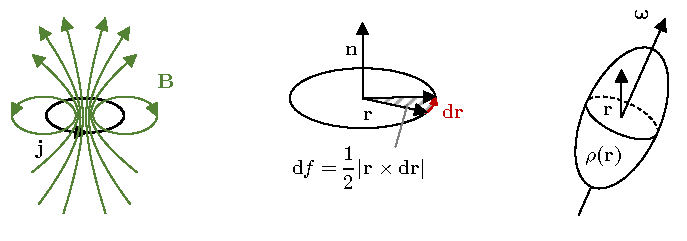
\includegraphics{magnetic_dipole_field_circle_conductor_ellipsoid.pdf}
	\caption{Links: Magnetfeld eines magnetischen Dipols, Mitte: Ein Kreisstrom erzeugt ein magnetisches Dipolmoment, rechts: starrer Körper, der mit $\vec\omega$ rotiert und einer Ladungsverteilung $\rho(\vec r)$ besitzt. }
	\label{fig:magnetic_dipole_field_circle_conductor_ellipsoid}
\end{figure}

Zuletzt betrachten wir einen starren geladenen Körper, der um eine Rotationsachse $\vec {\omega }$ rotiert (\Abbref{fig:magnetic_dipole_field_circle_conductor_ellipsoid}, rechts). Die lokale Geschwindigkeit für eine Ladung in diesem Körper ist $\vec {v}\left(\vec {r}\right)=\vec {\omega }\times \vec {r}$. Die rotierenden Ladungen resultieren in einer Stromdichte $\vec {j}=\rho \vec {v}$, sodass ein Dipolmoment induziert wird:
\begin{equation*}
	\vec {m}=\frac{1}{2}\int d^{3}\vec {r}\,\rho \left(\vec {r}\right)\vec {r}\times \vec {v}.
\end{equation*}
Gleichzeitig besitzt der Körper einen Drehimpuls
\begin{equation*}
	\vec {L}=\int \diffa[3]{\vec{r}}\rho _{m}\left(\vec {r}\right)\vec {r}\times \vec {v}.
\end{equation*}
Trifft man jetzt die Annahme, dass die Verteilungen von Ladung und Masse im Körper gleich sind,
\begin{equation*}
	\frac{\rho \left(\vec {r}\right)}{\rho _{m}\left(\vec {r}\right)}=\frac{q_{\mathrm{ges}}}{m_{\mathrm{ges}}}\equiv \frac{q}{M},
\end{equation*}
dann findet man eine Proportionalität von $\vec {m}$ und $\vec {L}$:
\begin{equation*}
	\vec {m}=\frac{q}{2M}\vec {L}
\end{equation*}
Der Proportionalitätsfaktor $\left| \vec {m}\right| /\left| \vec {L}\right| $ wird als gyromagnetisches Verhältnis bezeichnet. Für den Spin gibt es allerdings eine Abweichung, die aus der Relativitätstheorie hervorgeht und es gilt eigentlich
\begin{equation*}
	\vec {m}=g\frac{q}{2M}\vec {L}
\end{equation*}
mit einem zusätzlichen Landé-Faktor (oder g-Faktor), dessen Wert von der Teilchensorte abhängt. Für Elektronen ist $g\approx 2$, für Protonen $g\approx 2\cdot 2,79$ und für Neutronen $g\approx 2\cdot \left(-1,91\right)$.

Auch die Erde ist ein magnetischer Dipol, der durch Ströme im flüssigen äußeren Erdkern angetrieben wird. Bemerkenswerterweise ist die Dipolachse leicht gegen die Erdachse geneigt und die Polarität dreht sich rund alle 200.000 Jahre um. Der Mechanismus ist allerdings bis heute nicht genau verstanden.

\subsection{Kraft, Drehmoment und Energie}

Die bereits bekannte Kraft auf ein Volumen $V$ mit Stromverteilung $\vec {j}\left(\vec {r}\right)$
\begin{equation*}
	\vec {F}=\int \vec {j}\left(\vec {r}\right)\times \vec {B}\left(\vec {r}\right)\diffa[3]{\vec{r}}
\end{equation*}
lässt sich nach $\vec {B}$ um $\vec {r}=\vec {0}$ Taylor-entwickeln:
\begin{equation*}
	\vec {F}\approx \int \vec {j}\left(\vec {r}\right)\times \left(\vec {B}\left(0\right)+\vec {r}\cdot \nabla \vec {B}\left(0\right)+\ldots \right)\diffa[3]{\vec{r}}=\left(\vec {m}\times \nabla \right)\times \vec {B}\left(0\right)=\nabla \left(\vec {m}\cdot \vec {B}\right)
\end{equation*}
Die potentielle Energie eines Dipols $\vec {m}$ im magnetischen Feld $\vec {B}$ ergibt sich daraus durch Integration
\begin{equation*}
	\vec F=-\nabla U\implication U=-\vec {m}\cdot \vec {B}.
\end{equation*}
Das Minimum wird für $\vec {m} \upupharpoons \vec {B}$ erreicht\footnote{vgl. Funktionsweise von einem Kompass. }. $U$ enthält aber nicht die Energie um den Dipol $\vec {m}$ aufrechtzuerhalten!

Das Drehmoment hat die gleiche Form wie für elektrische Dipole,
\begin{equation*}
	\vec {M}=\vec {m}\times \vec {B}
\end{equation*}
und auch die Wechselwirkungsenergie für einen Dipol im Feld eines zweiten Dipols ist analog
\begin{equation*}
	U=-\frac{\mu _{0}}{4\pi }\frac{3\left(\vec {m}_{1}\cdot \hat{\vec {r}}\right)\left(\vec {m}_{2}\cdot \hat{\vec {r}}\right)-\vec {m}_{1}\cdot \vec {m}_{2}}{r^{3}}.
\end{equation*}



\section{Magnetische Felder in Materie}

Nun behandeln wir magnetische Felder in Materie. Die Vorgehensweise erfolgt analog zu den Kapiteln \ref{sec:mikroskopische_gleichungen_der_elektrostatik} und \ref{sec:Makroskopische_Gleichungen_der_Elektrostatik}. Die freien Ladungen bilden freie Ströme $j_{\mathrm{f}}\left(\vec {r},t\right)$ und gebundene Ladungen fügen jetzt noch gebundene Ströme hinzu $\vec {j}_{\mathrm{b}}\left(\vec {r},t\right)$. Außerdem werden auch magnetische Dipole durch den intrinsischen Spin der Teilchen hinzuaddiert. Die letzten beiden Quellen werden dann gemittelt über eine neue Größe beschrieben: die Magnetisierung.

\subsection{Einführung der Vakuumverschiebungsstromdichte}

In der Magnetostatik haben wir bisher nur
\begin{equation*}
	\nabla \times \vec {B}=\mu _{0}\vec {j},\quad\nabla \cdot \vec {j}=0
\end{equation*}
gehabt. Aber mit der vollständigen Kontinuitätsgleichung
\begin{equation*}
	\frac{\partial }{\partial t}\rho +\nabla \cdot \vec {j}=0
\end{equation*}
brauchen wir eine Verallgemeinerung, wenn $\nabla \cdot \vec {j}\neq 0$:
\begin{equation*}
	\nabla \times \vec {B}=\mu _{0}\vec {j}+\frac{1}{c^{2}}\frac{\partial \vec {E}}{\partial t}=\mu _{0}\left(\vec {j}+\varepsilon _{0}\frac{\partial \vec {E}}{\partial t}\right)
\end{equation*}
Das ist das Ampèresche Gesetz mit der Maxwellschen Verallgemeinerung.

\subsection{Einführung der Magnetisierung}

Wie für die Elektrostatik in Kapitel \ref{sec:mikroskopische_gleichungen_der_elektrostatik} und \ref{sec:Makroskopische_Gleichungen_der_Elektrostatik} beginnen wir, indem wir die mikroskopischen Gleichungen
\begin{equation*}
	\nabla\times \vec {b}=\mu _{0}\left(\vec {j}+\varepsilon _{0}\frac{\partial \vec {e}}{\partial t}\right), \quad\nabla\cdot \vec {b}=0
\end{equation*}
mitteln,
\begin{equation*}
	\vec {B}\left(\vec {r},t\right)=\left\langle \vec {b}\left(\vec {r},t\right)\right\rangle ,\quad \vec {E}\left(\vec {r},t\right)=\left\langle \vec {e}\left(\vec {r},t\right)\right\rangle .
\end{equation*}
Die Stromdichte
\begin{equation*}
	\vec {j}\left(\vec {r},t\right)=\vec {j}_{\mathrm{f}}\left(\vec {r},t\right)+\vec {j}_{\mathrm{b}}\left(\vec {r},t\right)
\end{equation*}
mit "`freien`` Strömen durch einzelne Ladungsträger mit Ladung $q_{i}$ und Geschwindigkeit $v_{i }$
\begin{equation*}
	\vec {j}_{\mathrm{f}}\left(\vec {r},t\right)=\sum _{i\left(f\right)}q_{i}\vec {v}_{i}\delta \left(\vec {r}-\vec {r}_{i}\left(t\right)\right)\implication \vec {j}_{\mathrm{F}}=\left\langle \vec {j}_{\mathrm{f}}\right\rangle .
\end{equation*}
Die gebundenen Ströme werden über alle Moleküle summiert, $\vec {j}_{\mathrm{b}}\left(\vec {r},t\right)=\sum _{n}\vec {j}_{n}\left(\vec {r},t\right)$ mit
\begin{equation*}
	\vec {j}_{n}\left(\vec {r},t\right)=\sum _{i\left(n\right)}q_{i}\vec {v}_{i}\delta \left(\vec {r}-\vec {r}_{i}\right)=\sum _{i\left(n\right)}q_{i}\left(\vec {v}_{n}+\vec {v}_{ni}\right)\delta \left(\vec {r}-\left(\vec {r}_{n}+\vec {r}_{ni}\right)\right)
\end{equation*}
und die Mittelung für das $n$-te Molekül ist (verwende wieder eine Glättungsfunktion $f$)
\begin{equation*}
	\left\langle \vec {j}_{n}\left(\vec {r},t\right)\right\rangle =\sum _{i\left(n\right)}q_{i}\left(\vec {v}_{n}+\vec {v}_{ni}\right)f\left(\vec {r}-\left(\vec {r}_{n}+\vec {r}_{ni}\right)\right).
\end{equation*}
Eine Taylor-Entwicklung um $\vec {r}_{n}$ liefert
\begin{equation*}
	\left\langle \vec {j}_{n}\left(\vec {r},t\right)\right\rangle =\sum _{i\left(n\right)}q_{i}\left(\vec {v}_{n}+\vec {v}_{ni}\right)\left[f\left(\vec {r}-\vec {r}_{n}\right)-\vec {r}_{ni}\cdot \nabla f\left(\vec {r}-\vec {r}_{n}\right)+\ldots \right].
\end{equation*}
Betrachte zunächst die Terme mit $\sum _{i\left(n\right)}q_{i}\vec {v}_{ni}$, die die molekularen Dipolmomente liefern. Der erste Term kann durch ein elektrisches Dipolmoment beschrieben werden:
\begin{equation*}
	\sum _{i\left(n\right)}q_{i}\vec {v}_{ni}=\sum _{i\left(n\right)}q_{i}\frac{\diff \vec {r}_{ni}}{\diff t}=\frac{\diff }{\diff t}\vec {p}_{n}
\end{equation*}
Der zweite Term enthält ein magnetisches Moment (verwende wieder die Tensorzerlegung in einen symmetrischen und einen asymmetrischen Anteil):
\begin{multline*}
	\sum _{i\left(n\right)}q_{i}\left(\vec {r}_{ni}\right)_{\beta }\left(\vec {v}_{ni}\right)_{\alpha }\\
	=\sum _{i\left(n\right)}\frac{1}{2}\left[q_{i}\left(\vec {r}_{ni}\right)_{\beta }\left(\vec {v}_{ni}\right)_{\alpha }-q_{i}\left(\vec {r}_{ni}\right)_{\alpha }\left(\vec {v}_{ni}\right)_{\beta }\right]+\sum _{i\left(n\right)}\frac{1}{2}\left[q_{i}\left(\vec {r}_{ni}\right)_{\beta }\left(\vec {v}_{ni}\right)_{\alpha }+q_{i}\left(\vec {r}_{ni}\right)_{\alpha }\left(\vec {v}_{ni}\right)_{\beta }\right],
\end{multline*}
wobei die Summanden der zweiten Summe verschwinden, weil diese Ströme jeweils auf ein Molekül beschränkt sind ($\nabla\cdot \vec {j}_{\mathrm{b}}=0$). Die erste Summe ist asymmetrisch und lässt sich als Kreuzprodukt schreiben,
\begin{equation*}
	\sum _{i\left(n\right)}q_{i}\left(\vec {r}_{ni}\right)_{\beta }\left(\vec {v}_{ni}\right)_{\alpha }=\frac{1}{2}\varepsilon _{\alpha \beta \gamma }\left(\sum _{i\left(n\right)}q_{i}\left(\vec {r}_{ni}\times \vec {v}_{ni}\right)\right)_{\gamma },
\end{equation*}
sodass sich ein sinnvolles molekulares magnetisches Dipolmoment ergibt,
\begin{equation*}
	\vec {m}_{n}=\frac{1}{2}\sum _{i\left(n\right)}q_{i}\left(\vec {r}_{ni}\times \vec {v}_{ni}\right).
\end{equation*}
Sammle nun alle bisher ausgewerteten Ausdrücke:
\begin{align*}
	\left\langle \left(\vec {j}_{n}\left(\vec {r},t\right)\right)_{\alpha }\right\rangle & =\left(\left(\sum _{i\left(n\right)}q_{i}\left(\vec {v}_{n}\right)_{\alpha }\right)+\frac{\diff }{\diff t}\left(\vec {p}_{n}\right)_{\alpha }\right)f\left(\vec {r}-\vec {r}_{n}\right)                                                                                                                                                                                                                 \\
	                                                                                     & \qquad-\left(\left(\sum _{i\left(n\right)}q_{i}\left(\vec {v}_{n}\right)_{\alpha }\left(\vec {r}_{ni}\right)_{\beta }\right)-\varepsilon _{\alpha \beta \gamma }\left(\vec {m}_{n}\right)_{\gamma }\right)\nabla _{\beta }f\left(\vec {r}-\vec {r}_{n}\right)                                                                                                                                           \\
	                                                                                     & =\left\langle q_{n}\left(\vec {v}_{n}\right)_{\alpha }\delta \left(\vec {r}-\vec {r}_{n}\right)\right\rangle +\frac{\partial }{\partial t}\left\langle \left(\vec {p}_{n}\right)_{\alpha }\delta \left(\vec {r}-\vec {r}_{n}\right)\right\rangle +\varepsilon _{\alpha \beta \gamma }\nabla _{\beta }\left\langle \left(\vec {m}_{n}\right)_{\gamma }\delta \left(\vec {r}-\vec {r}\right)\right\rangle \\
	                                                                                     & \qquad -\nabla _{\beta }\left\langle \left(\vec {v}_{n}\right)_{\alpha }\left(\vec {p}_{n}\right)_{\beta }\delta \left(\vec {r}-\vec {r}_{n}\right)\right\rangle
\end{align*}
Den letzten Term vernachlässigen wir im Folgenden als Term höherer Ordnung (Details sind im Buch von Jackson, Kap. 6.6, zu finden).

Mit diesen Ergebnissen erhalten wir jetzt schlussendlich die gemittelte Stromdichte der gebundenen Ladungen,
\begin{equation*}
	\left\langle \vec {j}_{\mathrm{b}}\left(\vec {r},t\right)\right\rangle =\sum _{n}\left\langle \vec {j}_{n}\left(\vec {r},t\right)\right\rangle =j_{\mathrm{M}}\left(\vec {r},t\right)+\frac{\partial }{\partial t}\vec {P}\left(\vec {r},t\right)+\nabla \times \vec {M}\left(\vec {r},t\right)
\end{equation*}
mit der Stromdichte der gebundenen Ladungen
\begin{equation*}
	\vec {j}_{\mathrm{M}}\left(\vec {r},t\right)=\left\langle \sum _{n}q_{n}\vec {v}_{n}\delta \left(\vec {r}-\vec {r}_{n}\right)\right\rangle ,
\end{equation*}
der makroskopischen Polarisation
\begin{equation*}
	\vec {P}\left(r,t\right)=\left\langle \sum _{n}\vec {p}_{n}\delta \left(\vec {r}-\vec {r}_{n}\right)\right\rangle
\end{equation*}
und der neu eingeführten Magnetisierung (Dichte der magnetischen Dipole)
\begin{equation*}
	\vec {M}\left(\vec {r},t\right)=\left\langle \sum _{n}\vec {m}_{n}\delta \left(\vec {r}-\vec {r}_{n}\right)\right\rangle .
\end{equation*}
Daraus ergibt sich die die gemittelte Stromdichte als Summe der makroskopischen und mikroskopischen Stromdichte,
\begin{equation*}
	\left\langle \vec {j}\left(\vec {r},t\right)\right\rangle =\left\langle \vec {j}_{\mathrm{f}}\left(\vec {r},t\right)\right\rangle +\left\langle \vec {j}_{\mathrm{b}}\left(\vec {r},t\right)\right\rangle =\underset{\vec {j}_{\mathrm{Ma}}}{\underbrace{\vec {j}_{\mathrm{F}}\left(\vec {r},t\right)+\vec {j}_{\mathrm{M}}\left(\vec {r},t\right)}}+\underset{\vec {j}_{\mathrm{Mi}}\left(\vec {r},t\right)}{\underbrace{\frac{\partial }{\partial t}\vec {P}\left(\vec {r},t\right)+\nabla \times \vec {M}\left(\vec {r},t\right)}}
\end{equation*}
und wir können die makroskopischen Feldgleichungen formulieren:
\begin{align*}
	\divg \vec {B} & =0                                                                                                                                                                                            \\
	\rot \vec {B}  & =\mu _{0}\left(\vec {j}_{\mathrm{Ma}}\left(\vec {r},t\right)+\vec {j}_{\mathrm{Mi}}\left(\vec {r},t\right)+\varepsilon _{0}\frac{\partial }{\partial t}\vec {E}\left(\vec {r},t\right)\right) \\
	               & =\mu _{0}\left(\vec {j}_{\mathrm{Ma}}\left(\vec {r},t\right)+\frac{\partial }{\partial t}\vec {D}\left(\vec {r},t\right)+\nabla \times \vec {M}\left(\vec {r},t\right)\right)
\end{align*}
Nun führen wir noch das magnetische Feld $\vec {H}$ ein,
\begin{equation*}
	\vec {H}\left(\vec {r},t\right)=\frac{1}{\mu _{0}}\vec {B}\left(\vec {r},t\right)-M\left(\vec {r},t\right)\equivalence \vec {B}\left(\vec {r},t\right)=\mu _{0}\left(H\left(\vec {r},t\right)+M\left(\vec {r},t\right)\right)
\end{equation*}
Die Magnetisierung $\vec {M}$ wird also wieder in ein Hilfsfeld integriert, was einen einfacheren Ausdruck für die zweite Feldgleichung erlaubt:
\begin{equation*}
	\boxed{\rot \vec {H}=\vec {j}_{\mathrm{Ma}}+\frac{\partial }{\partial t}\vec {D}}
\end{equation*}

\begin{formal}
	Die Wirbel des Magnetfelds $\vec {H}$ sind die makroskopische Stromdichte $\vec {j}_{\mathrm{Ma}}$ und der dielektrische Verschiebungsstrom $\partial _{t}\vec {D}$.
\end{formal}

Das fundamentale magnetische Feld ist die magnetische Flussdichte $\vec {B}$.


\subsection{Materialgesetze und Randbedingungen}

Wir haben bereits gesehen, dass die Felder $\vec {B}$ und $\vec {H}$ über die Magnetisierung in Beziehung stehen:
\begin{equation*}
	\vec {H}=\frac{1}{\mu _{0}}\vec {B}-\vec {M}.
\end{equation*}
Für den Fall, dass die Magnetisierung linear vom Magnetfeld abhängt, führen wir den (linearen) Tensor der magnetischen Suszeptibilität ein,
\begin{equation*}
	M_{i}=\left(\chi _{m}\right)_{ij}H_{j}.
\end{equation*}
Nur wegen der historischen Konvention drücken wir die Magnetisierung als $\vec {M}\left(\vec {H}\right)$ aus und nicht (sinnvollererweise) als $\vec {M}\left(\vec {B}\right)$. Wir schreiben dann also
\begin{equation*}
	\vec {B}=\mu \vec {H}, \mu =\mu _{0}\left(1+\chi _{m}\right)
\end{equation*}
mit dem Tensor der magnetischen Permeabilität $\mu $. Im Allgemeinen ist $\vec {M}\nparallel \vec {H}$.

Sind die Magnetfelder sogar isotrop, kann man einfach schreiben:
\begin{equation*}
	\vec {M}=\chi _{m}\vec {H}, \vec {B}=\mu \vec {H}=\mu _{0}\left(1+\chi _{m}\right)\vec {H}
\end{equation*}
und
\begin{equation*}
	\mu =\mu _{0}\left(1+\chi _{m}\right)\equiv \mu _{0}\mu _{r}.
\end{equation*}
Die dimensionslose Größe $\mu _{r}$ wird als relative Permeabilität bezeichnet.

Bemerkungen:
\begin{itemize}
	\item $\left| \mu _{r}-1\right| $ ist in der Regel in Größenordnungen von $10^{-6}$, also sehr klein.

	\item Bei $\mu _{r}>1$ bzw. $\chi >0$ liegt Paramagnetismus vor, $\vec {M}\parallel \vec {H}$, das heißt, die Ausrichtung der atomaren oder molekularen magnetischen Momente ist entlang $\vec {H}$.

	\item Für $\mu _{r}<1$ bzw. $\chi <0$ spricht man von Diamagnetismus, $\vec {M}\updownharpoons \vec {H}$.
\end{itemize}


Bei Ferromagnetismus gibt es eine permanente Magnetisierung, auch wenn kein Magnetfeld anliegt. Der Zusammenhang zwischen der magnetischen Flussdichte $\vec {B}$ und dem Magnetfeld $\vec {H}$ ist hier nicht linear, wie man an der sogenannten Hysteresekurve (siehe \Abbref{fig:hysterese}) sieht.

\begin{figure}[ht]
	\centering
	\tfighysterese
	\caption{Magnetische Hysterese: An ein zuerst unmagnetisches Material wird ein Feld $H$ angelegt und erhöht. Der Verlauf der magnetischen Flussdichte folgt der Kurve (1) und erreicht schließlich einen Sättigungswert $B_\mathrm{S}$ bei $H_\mathrm{S}$. Wird das Feld auf 0 verringert (Kurve (2)) bleibt eine Magnetisierung zurück (Remanenz). Ein entgegengesetztes Feld von der Stärke der Koerzitivfeldstärke $H_\mathrm{C}$ ist nötig, um die Restmagnetisierung aufzuheben. Jenseits dieser Feldstärke wird die Magnetisierung umgedreht und die Hysteresekurve umgekert durchlaufen. }
	\label{fig:hysterese}
\end{figure}
Zuerst ist das Material unmagnetisch (Punkt im Ursprung). Legt man nun ein Magnetfeld an und erhöht die Feldstärke, erhöht sich der magnetische Fluss im Material entlang der Kurve (1). Dieser wächst aber nicht unbegrenzt, da es schließlich zur Sättigung kommt. Die zugehörige Feldstärke heißt entsprechend Sättigungsfeldstärke $H_{\mathrm{S}}$ und $B_{\mathrm{S}}$ Sättigungswert. Wird nun das Feld wieder verringert, sinkt auch die Flussdichte entlang Kurve (2). Allerdings fällt $B$ nicht bis auf $0$ ab, sondern erreicht den Wert $B_{\mathrm{R}}$, die Remanenzflussdichte. Die Flussdichte fällt erst auf $0$, wenn eine gegengerichtete Koerzitivfeldstärke $H_{\mathrm{C}}$ angelegt wird.

Wir diskutieren nun die Randbedingungen, die im Wesentlichen die gleichen wie in der Elektrostatik sind.

\begin{figure}[ht]
	\centering
	\tfigGrenzflaecheMagnetic
	\caption{Beim Übergang zwischen Medien mit verschiedener Permeabilität ändern sich Magnetfeld und magnetische Flussdichte. Außerdem kann ein Flächenstrom $\vec k$ in der Grenzfläche fließen.
		Die Randbedingungen werden aus Anwendung des Satzes von Gauß auf eine kleine "`Dose`` und des Satzes von Stokes auf eine kleine Schleife, die jeweils einen Teil der Grenzfläche enthalten, hergeleitet. }
	\label{fig:grenzflaeche_magnetic}
\end{figure}

An einer Grenzfläche, wie in \Abbref{fig:grenzflaeche_magnetic} dargestellt, muss die Normalkomponente von $\vec {B}$ stetig sein, da
\begin{equation*}
	\divg \vec {B}=0\quad\xrightarrow[\text{Satz von Gau\ss }]{\text{Dose},\: \Delta  h\rightarrow 0}\quad\hat{\vec {n}}\cdot \left(\vec {B}^{\left(2\right)}-\vec {B}^{\left(1\right)}\right)=0\equivalence B_{\perp }^{\left(1\right)}=B_{\perp }^{\left(2\right)}.
\end{equation*}
Insbesondere ist für ein lineares, isotropes Material auch
\begin{equation*}
	\mu _{1}H_{\perp }^{\left(1\right)}=\mu _{2}H_{\perp }^{\left(2\right)}.
\end{equation*}
Für die Tangentialkomponente von $\vec {H}$ gilt:
\begin{align*}
	\rot \vec {H} & =\vec {j}_{\mathrm{Ma}}+\frac{\partial \vec {D}}{\partial t}\xrightarrow{\text{Schleife}} \int \rot \vec {H}\cdot \diff \vec {f}=\int \vec {H}\cdot \diff \vec {s}=\int \left(\vec {j}_{\mathrm{Ma}}+\frac{\partial \vec {D}}{\partial t}\right)\cdot \hat{\vec {m}}\diff \vec f \\
	              & \xrightarrow{\Delta  h\rightarrow 0}\hat{\vec {t}}\cdot \left(\vec {H}^{\left(2\right)}-\vec {H}^{\left(1\right)}\right)=H_{\parallel }^{\left(2\right)}-H_{\parallel }^{\left(1\right)}=\vec {k}\cdot \hat{\vec {m}}
\end{align*}
mit einem Flächenstrom $\vec {k}$, der noch in der Grenzfläche fließen kann.

Ist das zweite Material sehr leicht magnetisierbar, also $\mu _{2}$ sehr groß gegenüber $\mu _{1}$ und $H^{\left(1\right)}_\parallel\approx 0$, also $\vec {H}^{\left(1\right)}$ orthogonal auf der Grenzfläche (siehe \Abbref{fig:magnetic_refraction}), dann kann das Feld nicht in das zweite Material eindringen ($\vec H^{(2)}\approx 0$) und das letztere verhält sich wie ein elektrischer Leiter, dessen Oberfläche eine Äquipotentialfläche ist.

\begin{figure}[ht]
	\centering
	\tfigMagneticRefraction
	\caption{Treffen die Magnetfeldlinien senkrecht auf eine Grenzfläche zu einem Material mit sehr viel größerer Permeabilität, so dringt das Magnetfeld nicht wesentlich in das zweite Material ein. }
	\label{fig:magnetic_refraction}
\end{figure}

\subsection{Magnetische Skalarpotentiale und ihre Anwendungen}



In der Magnetostatik ist wie wir gesehen haben $\nabla \cdot \vec {B}=0$ und $\nabla \times \vec {H}=\vec {j}$.
\begin{itemize}
	\item Für ein homogenes, lineares Medium ohne Ströme ist $\nabla \times \vec {H}=0$ und wir können $\vec {H}$ als Potentialfeld eines magnetischen Skalarpotentials $\phi _{m}$ schreiben
	      \begin{equation*}
		      \vec {H}=-\nabla \phi _{m}
	      \end{equation*}
	      und mit $\vec {B}=\mu \vec {H}$ und $\nabla \cdot \vec {B}=0$ erhalten wir eine Laplace-Gleichung
	      \begin{equation*}
		      \nabla ^{2}\phi _{m}=0.
	      \end{equation*}
	      Für eine Stromschleife gilt zum Beispiel an einem Punkt $P$
	      \begin{equation*}
		      \phi _{m}\left(P\right)=-\frac{I\Omega  }{4\pi },
	      \end{equation*}
	      wobei $\Omega$ das eingeschlossene Raumwinkelelement ist, siehe \Abbref{fig:ConductorLoopWithRefPoint}.

	      \begin{figure}[htb]
		      \centering
		      \tfigConductorLoopWithRefPoint
		      \caption{Das magnetische Potential einer stromdurchflossenen Leiterschleife mit Fläche $F$ an einem Punkt $P$ ist proportional zu dem Raumwinkelelement, das durch die Projektion der Schleife auf den Punkt $P$ eingeschlossen wird. }
		      \label{fig:ConductorLoopWithRefPoint}
	      \end{figure}
	\item In einem harten Ferromagneten ist $\vec {M}$ vorgegeben und $\vec {j}=0$. Dann ist
	      \begin{equation*}
		      \nabla \cdot \vec {B}=\mu _{0}\nabla \cdot \left(\vec {H}+\vec {M}\right)=0,\quad \vec {H}=-\nabla \phi _{m}
	      \end{equation*}
	      und folglich
	      \begin{equation*}
		      \nabla ^{2}\phi _{m}=-\rho _{m},\quad \rho _{m}=-\nabla \cdot \vec {M}.
	      \end{equation*}
	      In einem Ferromagneten gilt also eine Poisson-Gleichung mit einer effektiven magnetischen Ladungsdichte $\rho _{m}$. Ohne Randflächen ist die Lösung einfach
	      \begin{equation*}
		      \phi _{m}=-\frac{1}{4\pi }\int \frac{\nabla '\cdot \vec {M}\left(\vec {r}'\right)}{\left| \vec {r}-\vec {r}'\right| }\diffa[3]{\vec{r}'}
	      \end{equation*}
	      und mit partieller Integration
	      \begin{equation*}
		      \phi _{m}=-\frac{1}{4\pi }\nabla \cdot \int \frac{\vec {M}\left(\vec {r}'\right)}{\left| \vec {r}-\vec {r}'\right| }\diffa[3]{\vec{r}'}.
	      \end{equation*}
	      Führt man eine Fernfeldentwicklung durch, $1/\left| \vec {r}-\vec {r}'\right| \approx 1/r$ und berücksichtigt nur den ersten Term, so erhält man
	      \begin{equation*}
		      \phi _{m}\left(\vec {r}\right)=-\frac{1}{4\pi }\nabla \left(\frac{1}{r}\right)\cdot \int \vec {M}\left(\vec {r}'\right)\diffa[3]{\vec{r}'}=\frac{1}{4\pi }\frac{\vec {m}\cdot \vec {r}}{r^{3}},
	      \end{equation*}
	      also ein Dipolfeld. Mit Randflächen ist
	      \begin{equation*}
		      \phi _{m}\left(\vec {r}\right)=-\frac{1}{4\pi }\int _{V}\frac{\nabla '\cdot \vec {M}\left(\vec {r}'\right)}{\left| \vec {r}-\vec {r}'\right| }\diffa[3]{\vec{r}'}+\frac{1}{4\pi }\oint _{\partial V}\frac{\vec {n}'\cdot \vec {M}\left(\vec {r}'\right)}{\left| \vec {r}-\vec {r}'\right| }\diff \vec {f}'.
	      \end{equation*}
	      Der Ausdruck $\vec {n}\cdot \vec {M}$ lässt sich als effektive magnetische Flächenladungsdichte $\sigma _{m}$ sehen. Ist die Magnetisierung homogen, dann ist das Potential nur von $\sigma _{m}$ abhängig.
\end{itemize}
Beispiele
\begin{itemize}
	\item Homogen magnetisierte Kugel:
	      \begin{equation*}
		      \phi _{m}\left(\vec {r}\right)=-\frac{1}{4\pi }\vec {M}\cdot \nabla \int _{V_{\mathrm{K}}}\frac{\diffa[3]{\vec{r}'}}{\left| \vec {r}-\vec {r}'\right| }=-\frac{1}{2}\vec {M}\cdot \nabla \int _{0}^{R}\int _{-1}^{1}\frac{r'^{2}\diff r'\diff \cos \vartheta '}{\sqrt{r^{2}+r'^{2}+2rr'\cos \vartheta '}}\diff \vartheta
	      \end{equation*}
	      Im Inneren der Kugel ($r<R$) ist das Ergebnis
	      \begin{equation*}
		      \phi _{m}\left(\vec {r}\right)=\frac{1}{3}\vec {M}\cdot \vec {r}, \quad\vec {H}_{\mathrm{i}}=-\nabla \phi _{m}=-\frac{1}{3}\vec {M},\quad \vec {B}_{\mathrm{i}}=\mu _{0}\left(\vec {H}_{\mathrm{i}}+\vec {M}\right)=\frac{2}{3}\mu _{0}\vec {M},
	      \end{equation*}
	      also $\vec {H}_{\mathrm{i}}\updownharpoons \vec {M}\upupharpoons \vec {B}_{\mathrm{i}}$.

	      Außerhalb der Kugel ist dagegen
	      \begin{equation*}
		      \phi _{m}\left(\vec {r}\right)=\frac{1}{4\pi }\frac{\vec {m}\cdot \vec {r}}{r^{3}},\quad \vec {m}=\frac{4}{3}\pi R^{3}\vec {M}
	      \end{equation*}
	      und
	      \begin{equation*}
		      H_{\mathrm{a}}=\frac{1}{\mu _{0}}\vec {B}_{\mathrm{a}}=-\nabla \phi _{m}
	      \end{equation*}
	      also wieder ein Dipolfeld. Magnetische Flussdichte und Magnetfeld sind in \Abbref{fig:magnetic_field_homogenously_magnetized_ball} dargestellt \textendash{} im Innern der Kugel ist das Magnetfeld entgegen der magnetischen Flussdichte gerichtet. Während $\vec {B}$ ein reines Wirbelfeld ist ($\divg \vec {B}=0$), weist $\vec {H}$ einen Sprung am Kugelrand auf und besitzt damit Quellen $\sigma _{m}=\vec {n}\cdot \vec {M}$.

	      \begin{figure}[htb]
		      \centering
		      \begin{tikzpicture}[
				      scale=.7,
				      mcolor/.style=legreen,
				      pics/graph/.style={background code={
								      \coordinate (O) at (0,0);
								      \coordinate (P) at (1,2);
								      \draw (O) circle [radius=1];
								      \foreach \vzx in {1,-1}{
										      \draw[midarrow] (\vzx*0.5,0.866) ..
										      controls ($1.2*(\vzx*0.5,0.866)$)
										      and (\vzx*1.2, 2.4) .. (\vzx*2.5,3);
										      \draw[midarrow] (\vzx*2.5,-3) ..
										      controls (\vzx*1.2,-2.4)
										      and ($1.2*(\vzx*0.5,-0.866)$) .. (\vzx*0.5,-0.866);
										      \draw[midarrow=.51] (\vzx*0.866,0.5)
										      .. controls +($.8*(\vzx*0.866,0.5)$)
										      and (\vzx*3,1)
										      .. (\vzx*3,0)
										      .. controls (\vzx*3,-1) and ($1.6*(\vzx*0.866,-0.5)$)
										      .. (\vzx*0.866,-0.5) ;
										      \draw[arr] (\vzx*0.866,#1*-0.4) -- (\vzx*0.866,#1*0.4);
										      \draw[arr] (\vzx*0.5,#1*-0.8) -- (\vzx*0.5,#1*0.8);
										      \draw[arr, mcolor] (\vzx*0.7,-0.4) -- +(0,0.8);
										      \draw[arr, mcolor] (\vzx*0.25,-0.4) -- +(0,0.8);
									      }
								      \draw[midarrow=.6] (0,1) -- (0,3.2);
								      \draw[midarrow=.4] (0,-3.2) -- (0,-1);
								      \draw[arr] (0,#1*-.9) -- (0,#1*0.9);
							      }}
			      ]

			      %\pic=1 at (0,0) [transform shape]{graph};
			      %\pic at (7,0) [transform shape]{graph};

			      \draw (0,0) pic[transform shape] {graph=1} node[outer sep=70,above] {$\vec B$-Feld};
			      \draw (7,0) pic[transform shape] {graph=-1} node[outer sep=70,above] {$\vec H$-Feld};
			      \node[mcolor] at (-1.5,0) {$\vec M$};
			      \node[mcolor] at (-1.5+7,0) {$\vec M$};
		      \end{tikzpicture}
		      \caption{Magnetisches Feld und magnetische Flussdichte einer homogen magnetisierten Kugel. Anders als die magnetische Flussdichte $B$ weist das Magnetfeld $H$ einen Sprung (Umpolung) an der Kugeloberfläche auf.  }
		      \label{fig:magnetic_field_homogenously_magnetized_ball}
	      \end{figure}

	\item Magnetisierbare Kugel im äußeren Feld $\vec {B}_{0}$:

	      Mit der Annahme, dass die Magnetisierung $\vec {M}=\left(\mu _{r}-1\right)\vec {H}_{\mathrm{i}}$ linear innerhalb des Kugelvolumens $V_{k}$ ist, erhält man durch Addition der Flussdichte $\vec {B}_{0}$
	      \begin{equation*}
		      \vec {B}_{\mathrm{i}}=\vec {B}_{0}+\frac{2}{3}\mu _{0}\vec {M},\quad \vec {H}_{\mathrm{i}}=\frac{1}{\mu _{0}}\vec {B}_{0}-\frac{1}{3}\vec {M}.
	      \end{equation*}
	      Ähnlich zur Elektrostatik beschreibt $-\vec {M}/3$ ein Entmagnetisierungsfeld. Mittels des linearen Materialgesetzes erhält man schließlich
	      \begin{equation*}
		      H_{\mathrm{i}}=\frac{1}{\mu _{0}}\frac{3}{\mu _{r}+2}\vec {B}_{0}
	      \end{equation*}
	      und
	      \begin{equation*}
		      \vec {M}=\frac{3}{\mu _{0}}\frac{\mu _{r}-1}{\mu _{r}+2}\vec {B}_{0}.
	      \end{equation*}
\end{itemize}

Beim Magnetismus ist alles analog zur Elektrizität AUSSER überall da, wo es genau anders rum ist

\section{Faradaysches Induktionsgesetz}

Bisher haben wir die Elektrostatik und die Magnetostatik getrennt betrachtet. Außerdem haben wir zwar bisher keine Zeitabhängigkeiten berücksichtigt, aber z.B. bereits gesehen, dass zeitabhängige Phänomene eine Rolle spielen, wie zum Beispiel in
\begin{equation*}
	\rot \vec {H}=\vec {j}+\frac{\partial \vec {D}}{\partial t}.
\end{equation*}
Solche sind unter anderem wichtig bei elektromagnetischen Wellen, dem Auf- und Abbau von Feldern etc.

\subsection{Integrale und differentielle Formulierung}

Die Entdeckung des Induktionsgesetzes durch Michael Faraday beruht auf der Beobachtung, dass durch eine Leiterschleife, das einem bewegten magnetischen Feld ausgesetzt ist, ein Strom fließt.

Wir betrachten im Folgenden ein Grundexperiment von Faraday, in dem ein Magnet in der Nähe einer Leiterschleife mit einer Geschwindigkeit $\vec v$ bewegt wird (siehe \Abbref{fig:inductionA}), sodass sich der magnetische Fluss durch die Schleife mit der Zeit ändert.

\begin{figure}
	\centering
	\tfigInductionA
	\caption{Ein Magnetfeld wird in der Nähe einer Leiterschleife $C=\partial F$ bewegt. Der sich ändernde magnetische Fluss bewirkt die Induktion einer Spannung in der Schleife und damit einen Induktionsstrom $I$. }
	\label{fig:inductionA}
\end{figure}

Wir bezeichnen die Leiterschleife als Randkurve $\partial F$ einer Fläche $F$ und führen zwei neue Größen ein: den magnetischen Fluss
\begin{equation*}
	\phi _{B}=\int _{F}\vec {B}\cdot \diff \vec {f}
\end{equation*}
und die elektrische Ringspannung entlang $\partial F$
\begin{equation*}
	Z_{E}=\int _{\partial F}\vec {E}\cdot \diff \vec {r}.
\end{equation*}
Die Ringspannung $Z_{E}$ bewirkt einen Stromfluss in der Schleife. Hiermit und aus den experimentellen Beobachtungen folgte ursprünglich die integrale Formulierung des Induktionsgesetzes
\begin{equation*}
	Z_{E}=-\frac{\diff }{\diff t}\phi _{B}\equivalence \int _{\partial F}\vec {E}\cdot \diff \vec {r}=-\frac{\diff }{\diff t}\int \vec {B}\cdot \diff \vec {f}.
\end{equation*}

\begin{formal}
	Die zeitliche Änderung des magnetischen Flusses durch eine Leiterschleife ruft eine Ringspannung und damit einen Strom hervor.
\end{formal}
Die Bedeutung des negativen Vorzeichens wird mit der Lenzschen Regel erklärt:
\begin{formal}
	Das induzierte elektrische Feld bzw. der induzierte elektrische Strom erzeugt ein Magnetfeld, das der Ursache der magnetischen Flussänderung entgegenwirkt.
\end{formal}
Mit dem Satz von Stokes kann das Induktionsgesetz auch differentiell ausgedrückt werden:
\begin{equation*}
	\rot \vec {E}=-\frac{\partial \vec {B}}{\partial t}
\end{equation*}

\begin{formal}
	Die Wirbel des elektrischen Feldes sind durch die Änderung der magnetischen Flussdichte bestimmt.
\end{formal}


\subsection{Bewegte Leiter}

Bisher haben wir den Leiter festgehalten und das Magnetfeld verändert. Als nächstes soll stattdessen der Leiter bewegt werden, wie in \Abbref{fig:inductionB} dargestellt.

\begin{figure}[ht]
	\centering
	\tfigInductionB
	\caption{Nun wird statt des Magnetfeldes die Leiterschleife mit der Geschwindigkeit $\vec v$ bewegt. }
	\label{fig:inductionB}
\end{figure}

Wir schreiben die treibende Ringspannung wieder als
\begin{equation}
	\label{eq:ringspannung_ruhesystem_leiter}
	Z_{E}=\int _{\partial F}\vec {E}'\cdot \diff \vec {r},
\end{equation}
aber jetzt wird das elektrische Feld im Ruhesystem des Leiters $\vec {E}'$ eingesetzt.

Die Physik soll nach Einsteins Relativitätstheorie in allen Inertialsystemen gleich sein. Eine Beschreibung des Versuchs im Ruhesystem des Leiters muss dasselbe Ergebnis liefern wie im Ruhesystem des Magnetfeldes. Dazu muss die Elektrodynamik invariant unter Lorentz-Transformationen sein. Für kleine Geschwindigkeiten gehen diese Transformationen in Galilei-Transformationen (vernachlässige für diesen Zweck Translationen in Raum und Zeit) $\vec {r}'=\vec {r}-vt$ über. Im Moment werden wir uns auf diese beschränken.

Für den magnetischen Fluss, der jetzt aus dem Integral über eine veränderliche Fläche $F\left(t\right)$ hervorgeht,
\begin{equation*}
	\frac{\diff }{\diff t}\phi _{B}=\frac{\diff }{\diff t}\int _{F\left(t\right)}\vec {B}\left(\vec {r},t\right)\cdot \diff \vec {f},
\end{equation*}
führen wir daher eine Galilei-Transformation durch
\begin{equation*}
	\frac{\diff }{\diff t}\phi _{B}=\frac{\diff }{\diff t}\int _{F}\vec {B}\left(\vec {r}'+\vec {v}t,t\right)\cdot \diff \vec {f}=\int _{F}\frac{\diff }{\diff t}\vec {B}\left(\underset{\vec {r}}{\underbrace{\vec {r}'+\vec {v}t}},t\right)\cdot \diff \vec {f}=\int _{F}\left(\frac{\partial }{\partial t}+\frac{\diff \vec {r}}{\diff t}\cdot \nabla _{\vec {r}}\right)\vec {B}\cdot \diff \vec {f}'.
\end{equation*}
Den zweiten Summanden im Integral schreiben wir um zu
\begin{equation*}
	\frac{\diff \vec {r}}{\diff t}\cdot \nabla _{\vec {r}}\vec {B}=\vec {v}\cdot \nabla _{\vec {r}}\vec {B}=-\nabla \times \left(\vec {v}\times \vec {B}\right)+\vec {v}\left(\nabla \cdot \vec {B}\right)
\end{equation*}
und erhalten
\begin{equation}
	\label{eq:dt_magn_potential}
	\frac{\diff }{\diff t}\phi _{B}=\int _{F}\left(\frac{\partial }{\partial t}-\nabla \times \left(\vec {v}\times \right)\right)\vec {B}\cdot \diff \vec {f}=\int _{F}\frac{\partial }{\partial t}\vec {B}\cdot \diff \vec {f}-\oint _{\partial F}\left(\vec {v}\times \vec {B}\right)\cdot \diff \vec {r}
\end{equation}
Diese Berechnungen wurden im Inertialsystem des Leiters durchgeführt. Nun soll zurück in das Laborsystem (Ruhesystem des Magnetfelds) transformiert werden. Wir wissen bereits, dass
\begin{equation*}
	Z_{e}=-\frac{\diff }{\diff t}\phi _{B}
\end{equation*}
gelten muss. Einsetzen der Gleichungen \eqref{eq:ringspannung_ruhesystem_leiter} und \eqref{eq:dt_magn_potential} führt auf
\begin{equation*}
	\int _{\partial F}\left(\vec {E}'-\vec {v}\times \vec {B}\right)\cdot \diff \vec {r}=-\int _{F}\frac{\partial }{\partial t}\vec {B}\cdot \diff \vec {f}
\end{equation*}
Daraus kann man das elektrische Feld im Laborsystem ablesen:
\begin{equation*}
	\vec {E}=\vec {E}'-\vec {v}\times \vec {B}
\end{equation*}
Dieses Ergebnis ist auch sinnvoll, weil $\rot \vec {E}=\partial _{t}\vec {B}$ erfüllt ist und außerdem die Lorentzkraft auf eine Ladung $q$ im Leiter
\begin{equation*}
	\vec {F}=q\vec {E}'=q\left(\vec {E}+\vec {v}\times \vec {B}\right)
\end{equation*}
ist (im Ruhesystem des Leiters bewegt sich $q$ nicht, im Laborsystem allerdings schon, und zwar mit $\vec {v}$).

\section{Energie des magnetischen Feldes und Induktivität}

\subsection{Energie eines statischen Magnetfeldes}

Die Energie von einem statischen Magnetfeld entspricht genau der Energie, die zum Aufbau des Feldes beim Einschalten des Stroms aufgebracht werden muss. Dabei entstehen aber auch temporäre elektrische Felder, sodass die Induktion berücksichtigt werden muss.

Die Arbeit pro Zeit $\diff _{t}U$, um den Strom $I$ bzw. die Stromdichte $\vec {j}$ aufrecht zu erhalten ist
\begin{equation*}
	\frac{\diff U}{\diff t}=-I\int _{C}\vec {E}\cdot \diff \vec {r}
\end{equation*}
Mit der integralen Formulierung des Induktionsgesetzes gilt also
\begin{equation*}
	\frac{\diff U}{\diff t}=I\frac{\diff }{\diff t}\int \vec {B}\cdot \diff \vec {f}
\end{equation*}
Damit kann man die Energiezunahme, die durch eine Änderung um $\delta \vec {B}$ bewirkt wird, schreiben als
\begin{equation*}
	\delta U=I\int \delta \vec {B}\cdot \diff \vec {f}=I\int \rot \left(\delta \vec {A}\right)\cdot \diff \vec {f}=I\int _{C}\delta \vec {A}\cdot \diff \vec {r}=\int \vec {j}\cdot \delta \vec {A}\diffa[3]{\vec{r}}=\int \left(\nabla \times \vec {H}\right)\cdot \delta \vec {A}\diffa[3]{\vec{r}}.
\end{equation*}
Der Anteil $\partial _{t}\vec {D}$ wird weggelassen, da dieser im Anfangs- und Endzustand gleich $0$ ist. Betrachte zunächst den Integranden
\begin{equation*}
	\left(\nabla \times \vec {H}\right)\cdot \delta \vec {A}=\nabla \cdot \left(\vec {H}\times \delta \vec {A}\right)+\vec {H}\cdot \left(\nabla \times \delta \vec {A}\right).
\end{equation*}
Der erste Summand verschwindet im Integral als Oberflächenterm. Es bleibt\footnote{Zur Erinnerung: In einem Dielektrikum gilt ganz äquivalent $\delta U_{\mathrm{el}}=\int \vec {E}\cdot \delta \vec {D}\diffa[3]{\vec{r}}$. }
\begin{equation*}
	\delta U=\int \vec {H}\cdot \delta \vec {B}\diffa[3]{\vec{r}},
\end{equation*}
bzw. in einem linearen Material
\begin{equation}
	\label{eq:magnetische_energie_linear}
	U=\frac{1}{2}\int \vec {H}\cdot \vec {B}\diffa[3]{\vec{r}}=\frac{1}{2}\int \vec {j}\cdot \vec {A}\diffa[3]{\vec{r}}.
\end{equation}
Alternativ kann man auch die Poisson-Gleichung
\begin{equation*}
	\nabla ^{2}\vec {A}=-\mu \vec {j}\implication \vec {A}=\frac{\mu }{4\pi }\int \frac{\vec {j}\left(\vec {r}'\right)}{\left| \vec {r}-\vec {r}'\right| }\diffa[3]{\vec{r}'}
\end{equation*}
aufstellen und erhält mit Gleichung \eqref{eq:magnetische_energie_linear}
\begin{equation*}
	U = \frac{\mu }{8\pi }\int \diffa[3]{\vec {r}'}\int \diffa[3]{\vec {r}}\frac{\vec {j}\left(\vec {r}\right)\cdot \vec {j}\left(\vec {r}'\right)}{\left| \vec {r}-\vec {r}'\right| }.
\end{equation*}

\subsection{Induktivität}

Mit den Erkenntnissen aus dem letzten Kapitel stellt sich die Frage, wie mehrere Leiterschleifen (wie z.B in \Abbref{fig:TwoInductors} dargestellt) miteinander wechselwirken.

\begin{figure}[ht]
	\centering
	\tfigTwoInductors
	\caption{Mehrere stromdurchflossene Leiterschleifen $C_i$ mit verschiedenen Induktivitäten $L_i$ beinflussen gegenseitig die Energie, die in den Magnetfeldern enthalten ist. }
	\label{fig:TwoInductors}
\end{figure}

Die Feldenergie zweier Leiterschleifen können wir schreiben als
\begin{equation*}
	U=\frac{1}{2}\sum _{i,k}L_{ik}I_{i}I_{k}
\end{equation*}
mit Selbstinduktivität $L_{ii}$ und Gegeninduktivität  $L_{ik},i\neq k$
\begin{align}
	\label{eq:selbstinduktivität}
	L_{ii} & =\frac{\mu }{4\pi }\frac{1}{I_{i}^{2}}\int \int \diffa[3]{\vec{r}}\diffa[3]{\vec{r}'}\frac{\vec {j}_{i}\left(\vec {r}\right)\cdot \vec {j}_{i}\left(\vec {r}'\right)}{\left| \vec {r}-\vec {r}'\right| } \\
	L_{ik} & =L_{ki}=\frac{\mu }{4\pi }\int _{C_{i}}\int _{C_{k}}\frac{\diff \vec {r}_{\mathrm{i}}\cdot \diff \vec {r}_{k}}{\left| \vec {r}-\vec {r}'\right| }
\end{align}
Es lässt sich nun bestimmen, welchen Fluss die Selbstinduktivität erzeugt:
\begin{equation*}
	\phi _{B}=\int \vec {B}\cdot \diff \vec {f}=\int \rot \vec {A}\cdot \diff \vec {f}=\oint _{\partial F}\vec {A}\cdot \diff \vec {r}=\frac{\mu }{4\pi }\oint _{\partial F}\int \frac{\vec {j}\left(\vec {r}'\right)\cdot \diff \vec {r}}{\left| \vec {r}-\vec {r}'\right| }\diffa[3]{\vec{r}'}\equiv LI
\end{equation*}
mit
\begin{equation*}
	L=\frac{\mu }{4\pi }\frac{1}{I}\oint _{\partial F}\int \frac{\vec {j}\left(\vec {r}'\right)\cdot \diff \vec {r}}{\left| \vec {r}-\vec {r}'\right| }\diffa[3]{\vec{r}'}.
\end{equation*}
Mit der Ersetzung $I\diff \vec {r}=\vec {j}\diffa[3]{\vec{r}}$ erhalten wir gerade die Gleichung \eqref{eq:selbstinduktivität}. Die Ringspannung entlang der Leiterschleife ist
\begin{equation*}
	V=\oint \vec {E}\cdot \diff \vec {r}=-\frac{\diff }{\diff t}\phi _{B}=-L\frac{\diff }{\diff t}I.
\end{equation*}
Führen wir eine Verallgemeinerung auf ein System von Leiterschleifen durch, erhalten wir die Ringspannung $V_{i}$ der Schleife $i$
\begin{equation*}
	V_{i}=\oint _{C_{i}}\vec {E}\cdot \diff \vec {r}=-\sum _{k}L_{ik}\frac{\diff }{\diff t}I_{k}.
\end{equation*}
Für einen geraden Draht mit Querschnittsradius $a$ und Länge $h$ (siehe \Abbref{fig:cylindricalConductorAndCoil} links) ist zum Beispiel
\begin{equation*}
	L=\frac{\mu }{2\pi }j\left(\ln \left(\frac{2h}{a}\right)-\frac{3}{4}\right)
\end{equation*}
und für eine unendliche lange Spule mit Querschnittsfläche $A$ und $N$ Windungen pro Länge $h$ (siehe \Abbref{fig:cylindricalConductorAndCoil} rechts)
\begin{equation*}
	L=\mu N^{2}\frac{A}{h},
\end{equation*}
denn $U=HBV/2=\mu H^{2}A/2$ mit $H=NI/h$ liefert
\begin{equation*}
	U=\frac{1}{2}\mu N^{2}I^{2}\frac{A}{h}
\end{equation*}
und
\begin{equation*}
	U=\frac{1}{2}LI^{2}.
\end{equation*}

\begin{figure}[htb]
	\centering
	\tfigcylindricalConductorAndCoil
	\caption{Links: Zylindrisches Drahtstück der Länge $h$ und Radius $a$ in einem Medium mit Permeabilität $\mu$. Rechts: Stück einer (eng gewickelten) Spule der Länge $h$. }
	\label{fig:cylindricalConductorAndCoil}
\end{figure}